% Compile: pdflatex main.tex && bibtex main && pdflatex main.tex && pdflatex main.tex
\documentclass{article}

\usepackage[preprint]{neurips_2026}

\usepackage[utf8]{inputenc}
\usepackage[T1]{fontenc}
\usepackage{hyperref}
\usepackage{url}
\usepackage{booktabs}
\usepackage{amsfonts}
\usepackage{amsmath}
\usepackage{amssymb}
\usepackage{amsthm}
\usepackage{nicefrac}
\usepackage{microtype}
\usepackage{xcolor}
\usepackage{graphicx}
\usepackage{float}

\newtheorem{lemma}{Lemma}
\raggedbottom
\setlength{\textfloatsep}{8pt plus 2pt minus 2pt}
\setlength{\floatsep}{6pt plus 2pt minus 2pt}
\setlength{\abovecaptionskip}{4pt}

% Generated by results/make_numbers.py. Do not edit by hand.

% ---- concrete: data and tuned configuration
% summary.json [concrete] n (rows in the data set)
\newcommand{\nConcreteN}{1{,}030}
% concrete.json d (features)
\newcommand{\nConcreteD}{8}
% summary.json [concrete] task (distribution)
\newcommand{\nConcreteTask}{normal}
% summary.json [concrete] picked.max_depth
\newcommand{\nConcretePickMaxDepth}{5}
% summary.json [concrete] picked.min_samples_leaf
\newcommand{\nConcretePickMinSamplesLeaf}{1}
% summary.json [concrete] picked.minibatch_frac
\newcommand{\nConcretePickMinibatchFrac}{0.8}
% summary.json [concrete] picked.learning_rate
\newcommand{\nConcretePickLearningRate}{0.0177}
% summary.json [concrete] picked.n_estimators
\newcommand{\nConcretePickNEstimators}{119}
% concrete.json search.n_trials
\newcommand{\nConcreteSearchTrials}{30}
% summary.json [concrete] tuned_constant_share, max over seeds, percent
\newcommand{\nConcreteTunedShareMax}{0}
% summary.json [concrete] default_constant_share, max over seeds, percent
\newcommand{\nConcreteDefaultShareMax}{0}
% summary.json [concrete] len(tuned_constant_share)
\newcommand{\nConcreteSeeds}{3}
% summary.json [concrete] tuned_test_nll, mean over seeds (nats)
\newcommand{\nConcreteTunedNLL}{2.925}

% ---- concrete: output equality over every fitted model
% summary.json [concrete] exact_all_models.fold_direct.n_rows
\newcommand{\nConcreteEqRows}{3{,}090}
% summary.json [concrete] exact_all_models.fold_direct.n_models
\newcommand{\nConcreteEqModels}{30}
% summary.json [concrete] exact_all_models.merged.bitwise_share, percent of rows
\newcommand{\nConcreteMergedBitwise}{80}
% summary.json [concrete] exact_all_models.merged.max_abs_diff (math mode)
\newcommand{\nConcreteMergedMaxDiff}{4.0\times 10^{-15}}

% ---- concrete: tuned one-row paired latency, ours (fold + direct) vs arm
% summary.json [concrete] tuned_paired.1.pristine.mean: mean over seeds of median log(t_ours/t_arm)
\newcommand{\nConcreteOnePristineLog}{$-$1.300}
% summary.json [concrete] tuned_paired.1.pristine.se: benchmark SE, sd/sqrt(3) over seed medians
\newcommand{\nConcreteOnePristineSE}{0.005}
% summary.json [concrete] tuned_paired.1.pristine.speedup_at_mean = exp(-mean)
\newcommand{\nConcreteOnePristineX}{3.67}
% raw concrete_latency_raw.json.gz tuned/seed*/1: paper's two-level bootstrap SE (seeds, then 10-rep blocks; 2,000 resamples)
\newcommand{\nConcreteOnePristineBootSE}{0.013}
% raw concrete_latency_raw.json.gz tuned/seed*/1: paper's two-level bootstrap 95% CI lower bound of the speedup
\newcommand{\nConcreteOnePristineBootLo}{3.61}
% raw concrete_latency_raw.json.gz tuned/seed*/1: paper's two-level bootstrap 95% CI upper bound of the speedup
\newcommand{\nConcreteOnePristineBootHi}{3.80}
% summary.json [concrete] tuned_paired.1.fold.mean: mean over seeds of median log(t_ours/t_arm)
\newcommand{\nConcreteOneFoldLog}{$-$1.344}
% summary.json [concrete] tuned_paired.1.fold.se: benchmark SE, sd/sqrt(3) over seed medians
\newcommand{\nConcreteOneFoldSE}{0.005}
% summary.json [concrete] tuned_paired.1.fold.speedup_at_mean = exp(-mean)
\newcommand{\nConcreteOneFoldX}{3.83}
% raw concrete_latency_raw.json.gz tuned/seed*/1: paper's two-level bootstrap SE (seeds, then 10-rep blocks; 2,000 resamples)
\newcommand{\nConcreteOneFoldBootSE}{0.012}
% raw concrete_latency_raw.json.gz tuned/seed*/1: paper's two-level bootstrap 95% CI lower bound of the speedup
\newcommand{\nConcreteOneFoldBootLo}{3.75}
% raw concrete_latency_raw.json.gz tuned/seed*/1: paper's two-level bootstrap 95% CI upper bound of the speedup
\newcommand{\nConcreteOneFoldBootHi}{3.94}
% summary.json [concrete] tuned_paired.1.direct.mean: mean over seeds of median log(t_ours/t_arm)
\newcommand{\nConcreteOneDirectLog}{$-$0.007}
% summary.json [concrete] tuned_paired.1.direct.se: benchmark SE, sd/sqrt(3) over seed medians
\newcommand{\nConcreteOneDirectSE}{0.005}
% summary.json [concrete] tuned_paired.1.direct.speedup_at_mean = exp(-mean)
\newcommand{\nConcreteOneDirectX}{1.01}
% raw concrete_latency_raw.json.gz tuned/seed*/1: paper's two-level bootstrap SE (seeds, then 10-rep blocks; 2,000 resamples)
\newcommand{\nConcreteOneDirectBootSE}{0.009}
% raw concrete_latency_raw.json.gz tuned/seed*/1: paper's two-level bootstrap 95% CI lower bound of the speedup
\newcommand{\nConcreteOneDirectBootLo}{0.99}
% raw concrete_latency_raw.json.gz tuned/seed*/1: paper's two-level bootstrap 95% CI upper bound of the speedup
\newcommand{\nConcreteOneDirectBootHi}{1.03}
% summary.json [concrete] tuned_paired.1.merged.mean: mean over seeds of median log(t_ours/t_arm)
\newcommand{\nConcreteOneMergedLog}{0.035}
% summary.json [concrete] tuned_paired.1.merged.se: benchmark SE, sd/sqrt(3) over seed medians
\newcommand{\nConcreteOneMergedSE}{0.004}
% summary.json [concrete] tuned_paired.1.merged.speedup_at_mean = exp(-mean)
\newcommand{\nConcreteOneMergedX}{0.97}
% raw concrete_latency_raw.json.gz tuned/seed*/1: paper's two-level bootstrap SE (seeds, then 10-rep blocks; 2,000 resamples)
\newcommand{\nConcreteOneMergedBootSE}{0.007}
% raw concrete_latency_raw.json.gz tuned/seed*/1: paper's two-level bootstrap 95% CI lower bound of the speedup
\newcommand{\nConcreteOneMergedBootLo}{0.95}
% raw concrete_latency_raw.json.gz tuned/seed*/1: paper's two-level bootstrap 95% CI upper bound of the speedup
\newcommand{\nConcreteOneMergedBootHi}{0.98}
% summary.json [concrete] tuned_paired.1.p50_ms.pristine, mean over seeds (ms)
\newcommand{\nConcreteOnePristineMs}{91.4}
% summary.json [concrete] tuned_paired.1.p50_ms.fold, mean over seeds (ms)
\newcommand{\nConcreteOneFoldMs}{96.5}
% summary.json [concrete] tuned_paired.1.p50_ms.direct, mean over seeds (ms)
\newcommand{\nConcreteOneDirectMs}{23.8}
% summary.json [concrete] tuned_paired.1.p50_ms.fold_direct, mean over seeds (ms)
\newcommand{\nConcreteOneOursMs}{23.8}
% summary.json [concrete] tuned_paired.1.p50_ms.merged, mean over seeds (ms)
\newcommand{\nConcreteOneMergedMs}{23.3}
% summary.json [concrete] tuned_paired.100.pristine.mean: mean over seeds of median log(t_ours/t_arm)
\newcommand{\nConcreteHundredPristineLog}{$-$1.372}
% summary.json [concrete] tuned_paired.100.pristine.se: benchmark SE, sd/sqrt(3) over seed medians
\newcommand{\nConcreteHundredPristineSE}{0.013}
% summary.json [concrete] tuned_paired.100.pristine.speedup_at_mean = exp(-mean)
\newcommand{\nConcreteHundredPristineX}{3.94}
% summary.json [concrete] tuned_paired.100.fold.mean: mean over seeds of median log(t_ours/t_arm)
\newcommand{\nConcreteHundredFoldLog}{$-$1.362}
% summary.json [concrete] tuned_paired.100.fold.se: benchmark SE, sd/sqrt(3) over seed medians
\newcommand{\nConcreteHundredFoldSE}{0.029}
% summary.json [concrete] tuned_paired.100.fold.speedup_at_mean = exp(-mean)
\newcommand{\nConcreteHundredFoldX}{3.90}
% summary.json [concrete] tuned_paired.100.direct.mean: mean over seeds of median log(t_ours/t_arm)
\newcommand{\nConcreteHundredDirectLog}{$-$0.008}
% summary.json [concrete] tuned_paired.100.direct.se: benchmark SE, sd/sqrt(3) over seed medians
\newcommand{\nConcreteHundredDirectSE}{0.009}
% summary.json [concrete] tuned_paired.100.direct.speedup_at_mean = exp(-mean)
\newcommand{\nConcreteHundredDirectX}{1.01}
% summary.json [concrete] tuned_paired.100.merged.mean: mean over seeds of median log(t_ours/t_arm)
\newcommand{\nConcreteHundredMergedLog}{0.007}
% summary.json [concrete] tuned_paired.100.merged.se: benchmark SE, sd/sqrt(3) over seed medians
\newcommand{\nConcreteHundredMergedSE}{0.005}
% summary.json [concrete] tuned_paired.100.merged.speedup_at_mean = exp(-mean)
\newcommand{\nConcreteHundredMergedX}{0.99}
% summary.json [concrete] tuned_paired.100.p50_ms.pristine, mean over seeds (ms)
\newcommand{\nConcreteHundredPristineMs}{105.5}
% summary.json [concrete] tuned_paired.100.p50_ms.fold, mean over seeds (ms)
\newcommand{\nConcreteHundredFoldMs}{104.9}
% summary.json [concrete] tuned_paired.100.p50_ms.direct, mean over seeds (ms)
\newcommand{\nConcreteHundredDirectMs}{24.7}
% summary.json [concrete] tuned_paired.100.p50_ms.fold_direct, mean over seeds (ms)
\newcommand{\nConcreteHundredOursMs}{24.8}
% summary.json [concrete] tuned_paired.100.p50_ms.merged, mean over seeds (ms)
\newcommand{\nConcreteHundredMergedMs}{24.7}
% concrete.json tuned[0].latency keys: full test set size
\newcommand{\nConcreteFullRows}{103}
% summary.json [concrete] tuned_paired.full.pristine.speedup_at_mean
\newcommand{\nConcreteFullPristineX}{3.81}
% summary.json [concrete] tuned_paired.1: t_fold/t_pristine = exp(d_pristine - d_fold), percent slower
\newcommand{\nConcreteFoldSlowerPct}{4}
% summary.json [concrete] plan_over_fit, median over tuned + default fits, percent of fit time
\newcommand{\nConcretePlanOverFit}{16}

% ---- yacht: data and tuned configuration
% summary.json [yacht] n (rows in the data set)
\newcommand{\nYachtN}{308}
% yacht.json d (features)
\newcommand{\nYachtD}{6}
% summary.json [yacht] task (distribution)
\newcommand{\nYachtTask}{normal}
% summary.json [yacht] picked.max_depth
\newcommand{\nYachtPickMaxDepth}{4}
% summary.json [yacht] picked.min_samples_leaf
\newcommand{\nYachtPickMinSamplesLeaf}{10}
% summary.json [yacht] picked.minibatch_frac
\newcommand{\nYachtPickMinibatchFrac}{0.8}
% summary.json [yacht] picked.learning_rate
\newcommand{\nYachtPickLearningRate}{0.0944}
% summary.json [yacht] picked.n_estimators
\newcommand{\nYachtPickNEstimators}{49}
% yacht.json search.n_trials
\newcommand{\nYachtSearchTrials}{20}
% summary.json [yacht] tuned_constant_share, max over seeds, percent
\newcommand{\nYachtTunedShareMax}{0}
% summary.json [yacht] default_constant_share, max over seeds, percent
\newcommand{\nYachtDefaultShareMax}{0}
% summary.json [yacht] len(tuned_constant_share)
\newcommand{\nYachtSeeds}{3}
% summary.json [yacht] tuned_test_nll, mean over seeds (nats)
\newcommand{\nYachtTunedNLL}{$-$0.934}

% ---- yacht: output equality over every fitted model
% summary.json [yacht] exact_all_models.fold_direct.n_rows
\newcommand{\nYachtEqRows}{904}
% summary.json [yacht] exact_all_models.fold_direct.n_models
\newcommand{\nYachtEqModels}{30}
% summary.json [yacht] exact_all_models.merged.bitwise_share, percent of rows
\newcommand{\nYachtMergedBitwise}{73}
% summary.json [yacht] exact_all_models.merged.max_abs_diff (math mode)
\newcommand{\nYachtMergedMaxDiff}{1.6\times 10^{-15}}

% ---- yacht: tuned one-row paired latency, ours (fold + direct) vs arm
% summary.json [yacht] tuned_paired.1.pristine.mean: mean over seeds of median log(t_ours/t_arm)
\newcommand{\nYachtOnePristineLog}{$-$1.280}
% summary.json [yacht] tuned_paired.1.pristine.se: benchmark SE, sd/sqrt(3) over seed medians
\newcommand{\nYachtOnePristineSE}{0.017}
% summary.json [yacht] tuned_paired.1.pristine.speedup_at_mean = exp(-mean)
\newcommand{\nYachtOnePristineX}{3.60}
% raw yacht_latency_raw.json.gz tuned/seed*/1: paper's two-level bootstrap SE (seeds, then 10-rep blocks; 2,000 resamples)
\newcommand{\nYachtOnePristineBootSE}{0.015}
% raw yacht_latency_raw.json.gz tuned/seed*/1: paper's two-level bootstrap 95% CI lower bound of the speedup
\newcommand{\nYachtOnePristineBootLo}{3.48}
% raw yacht_latency_raw.json.gz tuned/seed*/1: paper's two-level bootstrap 95% CI upper bound of the speedup
\newcommand{\nYachtOnePristineBootHi}{3.69}
% summary.json [yacht] tuned_paired.1.fold.mean: mean over seeds of median log(t_ours/t_arm)
\newcommand{\nYachtOneFoldLog}{$-$1.330}
% summary.json [yacht] tuned_paired.1.fold.se: benchmark SE, sd/sqrt(3) over seed medians
\newcommand{\nYachtOneFoldSE}{0.009}
% summary.json [yacht] tuned_paired.1.fold.speedup_at_mean = exp(-mean)
\newcommand{\nYachtOneFoldX}{3.78}
% raw yacht_latency_raw.json.gz tuned/seed*/1: paper's two-level bootstrap SE (seeds, then 10-rep blocks; 2,000 resamples)
\newcommand{\nYachtOneFoldBootSE}{0.013}
% raw yacht_latency_raw.json.gz tuned/seed*/1: paper's two-level bootstrap 95% CI lower bound of the speedup
\newcommand{\nYachtOneFoldBootLo}{3.68}
% raw yacht_latency_raw.json.gz tuned/seed*/1: paper's two-level bootstrap 95% CI upper bound of the speedup
\newcommand{\nYachtOneFoldBootHi}{3.87}
% summary.json [yacht] tuned_paired.1.direct.mean: mean over seeds of median log(t_ours/t_arm)
\newcommand{\nYachtOneDirectLog}{$-$0.005}
% summary.json [yacht] tuned_paired.1.direct.se: benchmark SE, sd/sqrt(3) over seed medians
\newcommand{\nYachtOneDirectSE}{0.004}
% summary.json [yacht] tuned_paired.1.direct.speedup_at_mean = exp(-mean)
\newcommand{\nYachtOneDirectX}{1.01}
% raw yacht_latency_raw.json.gz tuned/seed*/1: paper's two-level bootstrap SE (seeds, then 10-rep blocks; 2,000 resamples)
\newcommand{\nYachtOneDirectBootSE}{0.006}
% raw yacht_latency_raw.json.gz tuned/seed*/1: paper's two-level bootstrap 95% CI lower bound of the speedup
\newcommand{\nYachtOneDirectBootLo}{0.99}
% raw yacht_latency_raw.json.gz tuned/seed*/1: paper's two-level bootstrap 95% CI upper bound of the speedup
\newcommand{\nYachtOneDirectBootHi}{1.02}
% summary.json [yacht] tuned_paired.1.merged.mean: mean over seeds of median log(t_ours/t_arm)
\newcommand{\nYachtOneMergedLog}{0.039}
% summary.json [yacht] tuned_paired.1.merged.se: benchmark SE, sd/sqrt(3) over seed medians
\newcommand{\nYachtOneMergedSE}{0.002}
% summary.json [yacht] tuned_paired.1.merged.speedup_at_mean = exp(-mean)
\newcommand{\nYachtOneMergedX}{0.96}
% raw yacht_latency_raw.json.gz tuned/seed*/1: paper's two-level bootstrap SE (seeds, then 10-rep blocks; 2,000 resamples)
\newcommand{\nYachtOneMergedBootSE}{0.005}
% raw yacht_latency_raw.json.gz tuned/seed*/1: paper's two-level bootstrap 95% CI lower bound of the speedup
\newcommand{\nYachtOneMergedBootLo}{0.95}
% raw yacht_latency_raw.json.gz tuned/seed*/1: paper's two-level bootstrap 95% CI upper bound of the speedup
\newcommand{\nYachtOneMergedBootHi}{0.97}
% summary.json [yacht] tuned_paired.1.p50_ms.pristine, mean over seeds (ms)
\newcommand{\nYachtOnePristineMs}{36.0}
% summary.json [yacht] tuned_paired.1.p50_ms.fold, mean over seeds (ms)
\newcommand{\nYachtOneFoldMs}{37.2}
% summary.json [yacht] tuned_paired.1.p50_ms.direct, mean over seeds (ms)
\newcommand{\nYachtOneDirectMs}{9.7}
% summary.json [yacht] tuned_paired.1.p50_ms.fold_direct, mean over seeds (ms)
\newcommand{\nYachtOneOursMs}{9.7}
% summary.json [yacht] tuned_paired.1.p50_ms.merged, mean over seeds (ms)
\newcommand{\nYachtOneMergedMs}{9.4}
% yacht.json tuned[0].latency keys: full test set size
\newcommand{\nYachtFullRows}{30}
% summary.json [yacht] tuned_paired.full.pristine.speedup_at_mean
\newcommand{\nYachtFullPristineX}{3.86}
% summary.json [yacht] tuned_paired.1: t_fold/t_pristine = exp(d_pristine - d_fold), percent slower
\newcommand{\nYachtFoldSlowerPct}{5}
% summary.json [yacht] plan_over_fit, median over tuned + default fits, percent of fit time
\newcommand{\nYachtPlanOverFit}{18}

% ---- credit-g: data and tuned configuration
% summary.json [credit-g] n (rows in the data set)
\newcommand{\nCreditGN}{1{,}000}
% credit-g.json d (features)
\newcommand{\nCreditGD}{61}
% summary.json [credit-g] task (distribution)
\newcommand{\nCreditGTask}{bernoulli}
% summary.json [credit-g] picked.max_depth
\newcommand{\nCreditGPickMaxDepth}{1}
% summary.json [credit-g] picked.min_samples_leaf
\newcommand{\nCreditGPickMinSamplesLeaf}{20}
% summary.json [credit-g] picked.minibatch_frac
\newcommand{\nCreditGPickMinibatchFrac}{0.5}
% summary.json [credit-g] picked.learning_rate
\newcommand{\nCreditGPickLearningRate}{0.0316}
% summary.json [credit-g] picked.n_estimators
\newcommand{\nCreditGPickNEstimators}{234}
% credit-g.json search.n_trials
\newcommand{\nCreditGSearchTrials}{20}
% summary.json [credit-g] tuned_constant_share, max over seeds, percent
\newcommand{\nCreditGTunedShareMax}{0}
% summary.json [credit-g] default_constant_share, max over seeds, percent
\newcommand{\nCreditGDefaultShareMax}{0}
% summary.json [credit-g] len(tuned_constant_share)
\newcommand{\nCreditGSeeds}{3}
% summary.json [credit-g] tuned_test_nll, mean over seeds (nats)
\newcommand{\nCreditGTunedNLL}{0.459}

% ---- credit-g: output equality over every fitted model
% summary.json [credit-g] exact_all_models.fold_direct.n_rows
\newcommand{\nCreditGEqRows}{3{,}000}
% summary.json [credit-g] exact_all_models.fold_direct.n_models
\newcommand{\nCreditGEqModels}{30}
% summary.json [credit-g] exact_all_models.merged.bitwise_share, percent of rows
\newcommand{\nCreditGMergedBitwise}{80}
% summary.json [credit-g] exact_all_models.merged.max_abs_diff (math mode)
\newcommand{\nCreditGMergedMaxDiff}{1.1\times 10^{-15}}

% ---- credit-g: tuned one-row paired latency, ours (fold + direct) vs arm
% summary.json [credit-g] tuned_paired.1.pristine.mean: mean over seeds of median log(t_ours/t_arm)
\newcommand{\nCreditGOnePristineLog}{$-$1.254}
% summary.json [credit-g] tuned_paired.1.pristine.se: benchmark SE, sd/sqrt(3) over seed medians
\newcommand{\nCreditGOnePristineSE}{0.004}
% summary.json [credit-g] tuned_paired.1.pristine.speedup_at_mean = exp(-mean)
\newcommand{\nCreditGOnePristineX}{3.51}
% raw credit-g_latency_raw.json.gz tuned/seed*/1: paper's two-level bootstrap SE (seeds, then 10-rep blocks; 2,000 resamples)
\newcommand{\nCreditGOnePristineBootSE}{0.005}
% raw credit-g_latency_raw.json.gz tuned/seed*/1: paper's two-level bootstrap 95% CI lower bound of the speedup
\newcommand{\nCreditGOnePristineBootLo}{3.47}
% raw credit-g_latency_raw.json.gz tuned/seed*/1: paper's two-level bootstrap 95% CI upper bound of the speedup
\newcommand{\nCreditGOnePristineBootHi}{3.53}
% summary.json [credit-g] tuned_paired.1.fold.mean: mean over seeds of median log(t_ours/t_arm)
\newcommand{\nCreditGOneFoldLog}{$-$1.259}
% summary.json [credit-g] tuned_paired.1.fold.se: benchmark SE, sd/sqrt(3) over seed medians
\newcommand{\nCreditGOneFoldSE}{0.010}
% summary.json [credit-g] tuned_paired.1.fold.speedup_at_mean = exp(-mean)
\newcommand{\nCreditGOneFoldX}{3.52}
% raw credit-g_latency_raw.json.gz tuned/seed*/1: paper's two-level bootstrap SE (seeds, then 10-rep blocks; 2,000 resamples)
\newcommand{\nCreditGOneFoldBootSE}{0.008}
% raw credit-g_latency_raw.json.gz tuned/seed*/1: paper's two-level bootstrap 95% CI lower bound of the speedup
\newcommand{\nCreditGOneFoldBootLo}{3.46}
% raw credit-g_latency_raw.json.gz tuned/seed*/1: paper's two-level bootstrap 95% CI upper bound of the speedup
\newcommand{\nCreditGOneFoldBootHi}{3.57}
% summary.json [credit-g] tuned_paired.1.direct.mean: mean over seeds of median log(t_ours/t_arm)
\newcommand{\nCreditGOneDirectLog}{0.000}
% summary.json [credit-g] tuned_paired.1.direct.se: benchmark SE, sd/sqrt(3) over seed medians
\newcommand{\nCreditGOneDirectSE}{0.002}
% summary.json [credit-g] tuned_paired.1.direct.speedup_at_mean = exp(-mean)
\newcommand{\nCreditGOneDirectX}{1.00}
% raw credit-g_latency_raw.json.gz tuned/seed*/1: paper's two-level bootstrap SE (seeds, then 10-rep blocks; 2,000 resamples)
\newcommand{\nCreditGOneDirectBootSE}{0.004}
% raw credit-g_latency_raw.json.gz tuned/seed*/1: paper's two-level bootstrap 95% CI lower bound of the speedup
\newcommand{\nCreditGOneDirectBootLo}{0.99}
% raw credit-g_latency_raw.json.gz tuned/seed*/1: paper's two-level bootstrap 95% CI upper bound of the speedup
\newcommand{\nCreditGOneDirectBootHi}{1.00}
% summary.json [credit-g] tuned_paired.1.merged.mean: mean over seeds of median log(t_ours/t_arm)
\newcommand{\nCreditGOneMergedLog}{0.052}
% summary.json [credit-g] tuned_paired.1.merged.se: benchmark SE, sd/sqrt(3) over seed medians
\newcommand{\nCreditGOneMergedSE}{0.003}
% summary.json [credit-g] tuned_paired.1.merged.speedup_at_mean = exp(-mean)
\newcommand{\nCreditGOneMergedX}{0.95}
% raw credit-g_latency_raw.json.gz tuned/seed*/1: paper's two-level bootstrap SE (seeds, then 10-rep blocks; 2,000 resamples)
\newcommand{\nCreditGOneMergedBootSE}{0.006}
% raw credit-g_latency_raw.json.gz tuned/seed*/1: paper's two-level bootstrap 95% CI lower bound of the speedup
\newcommand{\nCreditGOneMergedBootLo}{0.94}
% raw credit-g_latency_raw.json.gz tuned/seed*/1: paper's two-level bootstrap 95% CI upper bound of the speedup
\newcommand{\nCreditGOneMergedBootHi}{0.96}
% summary.json [credit-g] tuned_paired.1.p50_ms.pristine, mean over seeds (ms)
\newcommand{\nCreditGOnePristineMs}{70.4}
% summary.json [credit-g] tuned_paired.1.p50_ms.fold, mean over seeds (ms)
\newcommand{\nCreditGOneFoldMs}{72.2}
% summary.json [credit-g] tuned_paired.1.p50_ms.direct, mean over seeds (ms)
\newcommand{\nCreditGOneDirectMs}{20.2}
% summary.json [credit-g] tuned_paired.1.p50_ms.fold_direct, mean over seeds (ms)
\newcommand{\nCreditGOneOursMs}{20.3}
% summary.json [credit-g] tuned_paired.1.p50_ms.merged, mean over seeds (ms)
\newcommand{\nCreditGOneMergedMs}{19.5}
% summary.json [credit-g] tuned_paired.100.pristine.mean: mean over seeds of median log(t_ours/t_arm)
\newcommand{\nCreditGHundredPristineLog}{$-$1.273}
% summary.json [credit-g] tuned_paired.100.pristine.se: benchmark SE, sd/sqrt(3) over seed medians
\newcommand{\nCreditGHundredPristineSE}{0.022}
% summary.json [credit-g] tuned_paired.100.pristine.speedup_at_mean = exp(-mean)
\newcommand{\nCreditGHundredPristineX}{3.57}
% summary.json [credit-g] tuned_paired.100.fold.mean: mean over seeds of median log(t_ours/t_arm)
\newcommand{\nCreditGHundredFoldLog}{$-$1.256}
% summary.json [credit-g] tuned_paired.100.fold.se: benchmark SE, sd/sqrt(3) over seed medians
\newcommand{\nCreditGHundredFoldSE}{0.003}
% summary.json [credit-g] tuned_paired.100.fold.speedup_at_mean = exp(-mean)
\newcommand{\nCreditGHundredFoldX}{3.51}
% summary.json [credit-g] tuned_paired.100.direct.mean: mean over seeds of median log(t_ours/t_arm)
\newcommand{\nCreditGHundredDirectLog}{$-$0.001}
% summary.json [credit-g] tuned_paired.100.direct.se: benchmark SE, sd/sqrt(3) over seed medians
\newcommand{\nCreditGHundredDirectSE}{0.003}
% summary.json [credit-g] tuned_paired.100.direct.speedup_at_mean = exp(-mean)
\newcommand{\nCreditGHundredDirectX}{1.00}
% summary.json [credit-g] tuned_paired.100.merged.mean: mean over seeds of median log(t_ours/t_arm)
\newcommand{\nCreditGHundredMergedLog}{0.048}
% summary.json [credit-g] tuned_paired.100.merged.se: benchmark SE, sd/sqrt(3) over seed medians
\newcommand{\nCreditGHundredMergedSE}{0.011}
% summary.json [credit-g] tuned_paired.100.merged.speedup_at_mean = exp(-mean)
\newcommand{\nCreditGHundredMergedX}{0.95}
% summary.json [credit-g] tuned_paired.100.p50_ms.pristine, mean over seeds (ms)
\newcommand{\nCreditGHundredPristineMs}{76.0}
% summary.json [credit-g] tuned_paired.100.p50_ms.fold, mean over seeds (ms)
\newcommand{\nCreditGHundredFoldMs}{77.0}
% summary.json [credit-g] tuned_paired.100.p50_ms.direct, mean over seeds (ms)
\newcommand{\nCreditGHundredDirectMs}{20.6}
% summary.json [credit-g] tuned_paired.100.p50_ms.fold_direct, mean over seeds (ms)
\newcommand{\nCreditGHundredOursMs}{20.7}
% summary.json [credit-g] tuned_paired.100.p50_ms.merged, mean over seeds (ms)
\newcommand{\nCreditGHundredMergedMs}{20.3}
% credit-g.json tuned[0].latency keys: full test set size
\newcommand{\nCreditGFullRows}{100}
% summary.json [credit-g] tuned_paired.100.pristine.speedup_at_mean
\newcommand{\nCreditGFullPristineX}{3.57}
% summary.json [credit-g] tuned_paired.1: t_fold/t_pristine = exp(d_pristine - d_fold), percent slower
\newcommand{\nCreditGFoldSlowerPct}{0}
% summary.json [credit-g] plan_over_fit, median over tuned + default fits, percent of fit time
\newcommand{\nCreditGPlanOverFit}{29}

% ---- totals over the three data sets
% sum of exact_all_models.fold_direct.n_rows
\newcommand{\nEqRowsTotal}{6{,}994}
% sum of exact_all_models.fold_direct.n_models
\newcommand{\nEqModelsTotal}{90}

% ---- grid (1 seed, split 0): where constant learners appear
% summary.json [concrete] grid: number of grid points
\newcommand{\nConcreteGridPoints}{24}
% summary.json [concrete] grid: points with constant_share == 1
\newcommand{\nConcreteGridDegenerate}{6}
% summary.json [concrete] grid: min test_nll over the grid (nats)
\newcommand{\nConcreteGridBestNLL}{2.88}
% summary.json [concrete] grid: mean test_nll over degenerate points (nats)
\newcommand{\nConcreteGridDegNLL}{4.23}
% summary.json [concrete] grid: min ours_vs_pristine at share 1, > 1 round
\newcommand{\nConcreteGridDegMinX}{4{,}897}
% summary.json [concrete] grid: max ours_vs_pristine at share 1, > 1 round
\newcommand{\nConcreteGridDegMaxX}{8{,}153}
% summary.json [concrete] grid: median fold_vs_pristine at share 0
\newcommand{\nConcreteGridSplitFoldX}{0.97}
% summary.json [concrete] grid: min ours_vs_pristine at share 0
\newcommand{\nConcreteGridSplitOursMinX}{3.23}
% summary.json [concrete] grid: max ours_vs_pristine at share 0
\newcommand{\nConcreteGridSplitOursMaxX}{4.69}
% summary.json [yacht] grid: number of grid points
\newcommand{\nYachtGridPoints}{24}
% summary.json [yacht] grid: points with constant_share == 1
\newcommand{\nYachtGridDegenerate}{10}
% summary.json [yacht] grid: min test_nll over the grid (nats)
\newcommand{\nYachtGridBestNLL}{$-$0.80}
% summary.json [yacht] grid: mean test_nll over degenerate points (nats)
\newcommand{\nYachtGridDegNLL}{2.07}
% summary.json [yacht] grid: min ours_vs_pristine at share 1, > 1 round
\newcommand{\nYachtGridDegMinX}{4{,}742}
% summary.json [yacht] grid: max ours_vs_pristine at share 1, > 1 round
\newcommand{\nYachtGridDegMaxX}{10{,}069}
% summary.json [yacht] grid: median fold_vs_pristine at share 0
\newcommand{\nYachtGridSplitFoldX}{0.98}
% summary.json [yacht] grid: min ours_vs_pristine at share 0
\newcommand{\nYachtGridSplitOursMinX}{3.04}
% summary.json [yacht] grid: max ours_vs_pristine at share 0
\newcommand{\nYachtGridSplitOursMaxX}{4.13}
% summary.json [yacht] grid: share-1 fits stopped after 1 round
\newcommand{\nYachtGridOneRoundN}{2}
% summary.json [yacht] grid: min ours_vs_pristine, 1-round fits
\newcommand{\nYachtGridOneRoundMinX}{7.00}
% summary.json [yacht] grid: max ours_vs_pristine, 1-round fits
\newcommand{\nYachtGridOneRoundMaxX}{7.81}
% summary.json [credit-g] grid: number of grid points
\newcommand{\nCreditGGridPoints}{24}
% summary.json [credit-g] grid: points with constant_share == 1
\newcommand{\nCreditGGridDegenerate}{6}
% summary.json [credit-g] grid: min test_nll over the grid (nats)
\newcommand{\nCreditGGridBestNLL}{0.48}
% summary.json [credit-g] grid: mean test_nll over degenerate points (nats)
\newcommand{\nCreditGGridDegNLL}{0.61}
% summary.json [credit-g] grid: min ours_vs_pristine at share 1, > 1 round
\newcommand{\nCreditGGridDegMinX}{964}
% summary.json [credit-g] grid: max ours_vs_pristine at share 1, > 1 round
\newcommand{\nCreditGGridDegMaxX}{1{,}842}
% summary.json [credit-g] grid: median fold_vs_pristine at share 0
\newcommand{\nCreditGGridSplitFoldX}{0.99}
% summary.json [credit-g] grid: min ours_vs_pristine at share 0
\newcommand{\nCreditGGridSplitOursMinX}{3.41}
% summary.json [credit-g] grid: max ours_vs_pristine at share 0
\newcommand{\nCreditGGridSplitOursMaxX}{3.73}
% sum of grid points with constant_share == 1
\newcommand{\nGridDegenerateTotal}{22}
% 3 data sets x 24 grid points
\newcommand{\nGridPointsTotal}{72}

% ---- low-signal variant (Friedman 1, signal scaled by a)
% low_signal_friedman1.json n_trials
\newcommand{\nLowTrials}{15}
% low_signal_friedman1.json: fits over both levels x 3 seeds
\newcommand{\nLowFits}{6}
% low_signal_friedman1.json fits constant_share min, %
\newcommand{\nLowShareMin}{100}
% low_signal_friedman1.json levels.*.fits[*].latency.1.paired.pristine.speedup_median, min over fits
\newcommand{\nLowMinX}{1{,}808}
% low_signal_friedman1.json levels.*.fits[*].latency.1.paired.pristine.speedup_median, max over fits
\newcommand{\nLowMaxX}{2{,}215}
% low_signal_friedman1.json levels.*.fits[*].latency.1.arms.pristine.p50_ms min (ms)
\newcommand{\nLowPristineMinMs}{320}
% low_signal_friedman1.json levels.*.fits[*].latency.1.arms.pristine.p50_ms max (ms)
\newcommand{\nLowPristineMaxMs}{394}
% low_signal_friedman1.json levels.*.fits[*].latency.1.arms.fold_direct.p50_ms median (ms)
\newcommand{\nLowOursMs}{0.18}
% low_signal_friedman1.json levels.*.fits[*].latency.1.arms.fold.p50_ms median (ms)
\newcommand{\nLowFoldMs}{0.16}
% low_signal_friedman1.json picked.min_samples_leaf
\newcommand{\nLowPickLeaf}{200}
% low_signal_friedman1.json picked.minibatch_frac
\newcommand{\nLowPickMinibatch}{0.5}
% low_signal_friedman1.json levels.*.fits[*].latency.1.paired.pristine.se min (block bootstrap, log ratio)
\newcommand{\nLowSEMin}{0.02}
% low_signal_friedman1.json levels.*.fits[*].latency.1.paired.pristine.se max
\newcommand{\nLowSEMax}{0.07}

% ---- one-SE selection variant: held-out NLL of the one-SE pick minus the best pick
% one_se.json [credit-g_n100] paired_test_nll.nll_one_se_minus_best (nats)
\newcommand{\nOneSECGDiff}{+0.020}
% one_se.json [credit-g_n100] paired_test_nll.se, per-example SD/sqrt(n)
\newcommand{\nOneSECGSE}{0.014}
% one_se.json [credit-g_n100] paired_test_nll.n test rows
\newcommand{\nOneSECGN}{100}
% one_se.json [credit-g_n100] fits one_se_constant_share min, %
\newcommand{\nOneSECGShare}{100}
% one_se.json [friedman1_a0.0] paired_test_nll.nll_one_se_minus_best (nats)
\newcommand{\nOneSEFADiff}{$-$0.00012}
% one_se.json [friedman1_a0.0] paired_test_nll.se, per-example SD/sqrt(n)
\newcommand{\nOneSEFASE}{0.00016}
% one_se.json [friedman1_a0.0] paired_test_nll.n test rows
\newcommand{\nOneSEFAN}{200}
% one_se.json [friedman1_a0.0] fits one_se_constant_share min, %
\newcommand{\nOneSEFAShare}{100}
% one_se.json [friedman1_a0.1] paired_test_nll.nll_one_se_minus_best (nats)
\newcommand{\nOneSEFBDiff}{$-$0.00011}
% one_se.json [friedman1_a0.1] paired_test_nll.se, per-example SD/sqrt(n)
\newcommand{\nOneSEFBSE}{0.00012}
% one_se.json [friedman1_a0.1] paired_test_nll.n test rows
\newcommand{\nOneSEFBN}{200}
% one_se.json [friedman1_a0.1] fits one_se_constant_share min, %
\newcommand{\nOneSEFBShare}{100}
% one_se.json credit-g_n100 one_se_vs_best_1row_ms[0] mean
\newcommand{\nOneSECGOneSEMs}{0.12}
% one_se.json credit-g_n100 one_se_vs_best_1row_ms[1] mean
\newcommand{\nOneSECGBestMs}{0.45}

% ---- small-n variant (credit-g, 100 training rows)
% small_n_credit-g.json sizes.100.picked.min_samples_leaf
\newcommand{\nSmallPickLeaf}{10}
% small_n_credit-g.json sizes.100.picked.max_depth
\newcommand{\nSmallPickDepth}{4}
% small_n_credit-g.json sizes.100.picked.n_estimators
\newcommand{\nSmallPickRounds}{3}
% small_n_credit-g.json sizes.100.fits constant_share max, %
\newcommand{\nSmallShareMax}{0}
% small_n_credit-g.json sizes.100.fits latency.1.paired.pristine.speedup_median, mean
\newcommand{\nSmallX}{2.50}

% ---- environment
% concrete.json versions.ngboost
\newcommand{\nVerNgboost}{0.5.11}
% concrete.json versions.sklearn
\newcommand{\nVerSklearn}{1.9.1}
% concrete.json versions.numpy
\newcommand{\nVerNumpy}{2.5.4}
% concrete.json versions.python
\newcommand{\nVerPython}{3.12.3}
% summary.json [*] load (1-min load average), min
\newcommand{\nLoadMin}{7}
% summary.json [*] load, max
\newcommand{\nLoadMax}{20}
% summary.json [*] wall_s summed (s)
\newcommand{\nWallTuned}{5{,}451}

% ---- one external deployment (the only permitted sentence)
% PRIVATE_LINE.txt, verbatim; cite at most once
\newcommand{\nExternalLine}{On a proprietary binary forecasting task, a tuned NGBoost model (a seed ensemble of 8 models, three-parameter distribution) had every base learner constant because its tuned leaf size exceeded half the minibatch. Folding reduced single-row prediction for the ensemble from 1,338 ms to 29 ms p50 (46x; 5th-percentile per-call ratio 24.6x; a loaded 8-core host) with bit-identical outputs on every held-out row. On a tuned configuration whose trees split on two of three parameters (one third of learners constant), the gain was 1.37x, also bit-identical. This is one deployment, not a benchmark; the per-call times were not retained, so no paired SE beyond the per-call quantile is available.}

% ---- setup: design constants of the benchmark
% number of public data sets in summary.json
\newcommand{\nDataSets}{3}
% concrete.json search.n_folds
\newcommand{\nCVFolds}{3}
% concrete.json tuned[0].latency.1 arms n
\newcommand{\nRepsOne}{100}
% concrete.json tuned[0].latency.100 arms n
\newcommand{\nRepsHundred}{50}
% concrete.json tuned[0].latency key '100' (batch rows)
\newcommand{\nHundredRows}{100}
% concrete.json grid[0].latency.1 arms n
\newcommand{\nGridRepsOne}{15}
% concrete.json grid config.min_samples_leaf values
\newcommand{\nGridLeafValues}{1, 20, 100, 400}
% concrete.json grid config.minibatch_frac values
\newcommand{\nGridMinibatchValues}{0.2, 0.5, 1.0}
% concrete.json grid config.max_depth values
\newcommand{\nGridDepthValues}{1, 3}
% concrete.json grid config.n_estimators
\newcommand{\nGridRounds}{500}
% concrete.json grid config.learning_rate
\newcommand{\nGridLR}{0.01}
% concrete.json default[0].config.max_depth
\newcommand{\nDefaultDepth}{3}
% concrete.json default[0].config.min_samples_leaf
\newcommand{\nDefaultLeaf}{1}
% numlib/boot.py BLOCK (moving-block length, repetitions)
\newcommand{\nBlockLen}{10}
% numlib/boot.py two_level resamples default
\newcommand{\nBootResamples}{2{,}000}
% low_signal_friedman1.json fits[0].latency.1 arms n
\newcommand{\nLowReps}{60}
% low_signal_friedman1.json fits[0].per_param[0].batch_rows
\newcommand{\nLowBatchRows}{200}
% low_signal_friedman1.json fits[0].per_param[0].min_rows
\newcommand{\nLowMinRows}{400}
% low_signal_friedman1.json number of signal levels
\newcommand{\nLowLevels}{2}
% arms besides upstream: fold, direct, fold_direct, merged (summary.json tuned_paired)
\newcommand{\nArmsTried}{4}
% bench/results/variants/*.json count
\newcommand{\nVariantsTried}{3}
% SCOPE.md 'shared N-core host'
\newcommand{\nCores}{8}

% ---- variants: training rows; provenance
% low_signal_friedman1.json per_param[0].batch_rows / picked.minibatch_frac
\newcommand{\nLowTrainRows}{400}
% small_n_credit-g.json sizes key (training rows)
\newcommand{\nSmallTrainRows}{100}
% git rev-parse --short HEAD of the ngbfast repository
\newcommand{\nCommit}{d8dda3e}
% wc -l patches/ngboost-fold-constant-trees.patch
\newcommand{\nPatchLines}{393}
% raw latency dir used: True
\newcommand{\nRawBoot}{yes}


\newcommand{\fsub}{\ominus}
\newcommand{\fmul}{\otimes}

\title{Folding constant learners in NGBoost: bit-identical predictions, faster inference}

\author{%
  Moussa Ouallaf \\
}

\begin{document}

\maketitle

\begin{abstract}
NGBoost, a boosting method that predicts a full probability distribution, calls every stored tree on every prediction, even a tree that returns the same value for every input.
We fold such constant learners into a precomputed start value without changing the floating-point order, so outputs stay bit-identical, and we call the remaining trees directly on a float32 copy of the input that is checked once per call.
Against pristine ngboost \nVerNgboost{}, one-row prediction on tuned models was \nConcreteOnePristineX$\times$ faster on concrete (paired log ratio \nConcreteOnePristineLog{} $\pm$ \nConcreteOnePristineSE{} SE over \nConcreteSeeds{} seeds), \nYachtOnePristineX$\times$ on yacht and \nCreditGOnePristineX$\times$ on credit-g, with bit-identical outputs on all \nEqRowsTotal{} test rows of \nEqModelsTotal{} fitted models.
The tuned models had no constant learners, so that gain is direct traversal alone: ours against direct traversal only is a tie (concrete \nConcreteOneDirectLog{} $\pm$ \nConcreteOneDirectSE), and folding pays off only when the data carry no usable signal, where the search picked an all-constant model and one-row prediction was \nLowMinX$\times$ to \nLowMaxX$\times$ faster.
The evidence is \nDataSets{} public data sets with \nConcreteSeeds{} seeded splits each, every arm timed interleaved on the same fitted model on a shared, loaded \nCores-core host.
\end{abstract}

\section{Problem}
\label{sec:problem}

NGBoost \citep{duan2020ngboost} fits one regression tree per distribution parameter per boosting round, following the natural gradient (the gradient rescaled to the distribution's geometry, \citealp{amari1998natural}).
Prediction sums all those trees:
\begin{equation}
\theta_k(x) \;=\; \theta_{0,k} \;-\; \sum_{i=1}^{M} \big(\eta\, f_{ik}(x_{c_i})\big)\,\rho_i, \qquad k = 1,\dots,P.
\label{eq:pred}
\end{equation}
\begin{center}\small
\begin{tabular}{@{}ll@{\qquad}ll@{}}
\toprule
Symbol & Meaning & Symbol & Meaning\\
\midrule
$\theta_k(x)$ & parameter $k$ of the predicted distribution & $\eta$ & learning rate\\
$\theta_{0,k}$ & initial value of parameter $k$ & $\rho_i$ & line-search scale of round $i$\\
$f_{ik}$ & base learner (a CART tree) of round $i$, parameter $k$ & $c_i$ & feature columns sampled in round $i$\\
$M$, $P$ & number of rounds, number of parameters & & \\
\bottomrule
\end{tabular}
\end{center}
The upstream library \citep{ngboost_software} evaluates Equation~\eqref{eq:pred} as a loop that calls scikit-learn's \texttt{predict} \citep{pedregosa2011sklearn} $M P$ times.
Each call re-validates the input (array checks, a float32 cast, a feature count).
For a single row this validation costs more than walking the tree.

The loop also pays for trees that do nothing.
A tree with one node, a root-only tree, returns the same value for every input, but it still costs a full \texttt{predict} call.
This happens when no split is feasible: every round's tree is fitted on a minibatch, and when that minibatch is smaller than twice the minimum leaf size, the tree cannot split.
A tuning search can land there without any error, because under cross-validation the bound applies to the smaller training fold.
The model then predicts one fixed distribution for every input, yet one prediction still runs $M P$ calls.

\section{The change}
\label{sec:change}

The change has two parts, and both keep every output bit for bit the same as upstream.
Write $a \fsub b$ and $a \fmul b$ for float64 subtraction and multiplication with IEEE rounding \citep{goldberg1991floating}.
Upstream runs, for each column $k$ and round $i$ in order,
\begin{equation}
\theta_k^{(i)} = \theta_k^{(i-1)} \fsub \big((\eta \fmul f_{ik}(x_{c_i})) \fmul \rho_i\big), \qquad \theta_k^{(0)} = \theta_{0,k}.
\label{eq:loop}
\end{equation}

\textbf{Folding.} Call learner $(i,k)$ constant when $f_{ik}(x) = v_{ik}$ for every input the model accepts: a one-node tree, a tree whose leaves all hold the same value, or a \texttt{DummyRegressor}. Its update is then the scalar $s_{ik} = (\eta \fmul v_{ik}) \fmul \rho_i$. Let $i^*_k$ be the first round in which column $k$ has an input-dependent learner. The fold plan stores
\begin{equation}
\text{start}_k = \big(\cdots\big((\theta_{0,k} \fsub s_{1k}) \fsub s_{2k}\big) \cdots\big) \fsub s_{i^*_k - 1,\,k},
\label{eq:start}
\end{equation}
and, from round $i^*_k$ on, an ordered list of tree steps (Equation~\eqref{eq:loop}) and scalar steps $\theta_k \leftarrow \theta_k \fsub s_{ik}$.
Scalar steps after the first split are never merged: merging would reorder floating-point subtractions and change the last bit.
Prediction broadcasts $\text{start}$ to all rows and walks the list.
The number of learner calls falls from $MP$ to the number of input-dependent learners $N_s$; with $N_s = 0$ prediction is one broadcast.

\textbf{Direct traversal.} The input is validated and cast to float32 once per call. Each remaining tree is then walked with scikit-learn's low-level \texttt{tree\_.predict} with input checks off. Upstream \texttt{predict} performs the same cast and the same walk, so the values are equal.

\begin{lemma}[Folding is bit-identical]
\label{lem:fold}
For every fitted model and every row $x$ that upstream accepts, folded prediction with direct traversal returns the same float64 bits as Equation~\eqref{eq:loop} after round $M$, and it rejects exactly the rows that upstream rejects.
\end{lemma}

\begin{lemma}[When no tree can split]
\label{lem:bound}
Let each round fit its trees on $m = \lfloor \phi\, n' \rfloor$ rows, with minibatch fraction $\phi$ and $n'$ training rows after any early-stopping hold-out. If $m < \max(\text{min\_samples\_split},\, 2L)$, with $L$ the minimum leaf size, every learner is a one-node tree and $\theta(x) = \text{start}$ for every $x$: the model is one fixed distribution.
\end{lemma}

Both proofs are in Appendix~\ref{app:proofs}.
Lemma~\ref{lem:fold} rests on two facts: before $i^*_k$ the upstream value does not depend on $x$, and after it both paths apply the same rounded operations to the same operands in the same order.
For the rejection part, the plan probes every skipped learner once on a zero row, a NaN row and an infinity row, and folded prediction rejects the same inputs.
Lemma~\ref{lem:bound} turns into a fit-time warning that names the bound.
The upstream-ready patch for ngboost \nVerNgboost{} is \nPatchLines{} diff lines including tests; rounds stay stored, so staged prediction, feature importances and further \texttt{partial\_fit} calls are unchanged.

\section{Setup}
\label{sec:setup}

\textbf{Data.} Concrete \citep{yeh1998concrete} (\nConcreteN{} rows, \nConcreteD{} features) and yacht (\nYachtN{} rows, \nYachtD{} features) from the UCI collection \citep{dua2019uci}, with the test masks used for NGBoost's own benchmark \citep{hernandez2015probabilistic,duan2020ngboost}, as Normal regressions; credit-g from OpenML \citep{vanschoren2014openml} (\nCreditGN{} rows, \nCreditGD{} encoded features) as a Bernoulli classification. Each data set has \nConcreteSeeds{} splits, split $s$ fitted with seed $s$. Test rows are never used for fitting or tuning.

\textbf{Models.} A random search (\nConcreteSearchTrials{} trials on concrete, \nYachtSearchTrials{} on yacht and credit-g, \nCVFolds-fold cross-validated negative log-likelihood (NLL, lower is a better fit)) picks depth, leaf size, minibatch fraction, learning rate and the number of rounds on split~0's training rows. We also fit ngboost's default tree (depth \nDefaultDepth, leaf \nDefaultLeaf) and a grid of leaf sizes \{\nGridLeafValues\} $\times$ minibatch fractions \{\nGridMinibatchValues\} $\times$ depths \{\nGridDepthValues\} with \nGridRounds{} rounds.

\textbf{Arms.} All arms predict from the same fitted model, so data, features and tuning are equal by construction: pristine ngboost \nVerNgboost{} (the baseline), fold only, direct traversal only, ours (fold plus direct traversal), and an inexact ablation that merges all scalar steps of a column.

\textbf{Metrics.} Equality is checked bit for bit against upstream \texttt{pred\_param} on every test row of every fitted model. For latency the arms run interleaved in a rotating order, \nRepsOne{} repetitions for one row and \nRepsHundred{} for \nHundredRows{} rows. Per repetition $r$ the paired statistic is
\begin{equation}
d_r = \log t^{\text{ours}}_r - \log t^{\text{arm}}_r, \qquad \text{speedup} = \exp(-\bar d),
\label{eq:ratio}
\end{equation}
where $\bar d$ is the mean over seeds of the per-seed median of $d_r$; negative $d$ means ours is faster. The benchmark SE is the standard deviation of the per-seed medians over $\sqrt{3}$. We add a two-level bootstrap \citep{lahiri2003resampling} that resamples seeds, then moving blocks of \nBlockLen{} consecutive repetitions (consecutive timings share machine load), with \nBootResamples{} resamples. A difference inside its SE is called a tie.

\textbf{Variants tried.} We ran \nArmsTried{} arms against upstream and \nVariantsTried{} follow-up settings. The arms, the grid and the tuned and default configurations were fixed in a written plan before any run. The follow-ups (small data, low signal, one-SE model selection) were added after the tuned models came out with no constant learners, so they are post hoc.

\section{Results}
\label{sec:results}

\textbf{Equality holds everywhere.} Fold only, direct traversal only and ours returned the same bits as upstream on all \nEqRowsTotal{} test rows of \nEqModelsTotal{} fitted models (concrete \nConcreteEqRows{} rows / \nConcreteEqModels{} models, yacht \nYachtEqRows{} / \nYachtEqModels, credit-g \nCreditGEqRows{} / \nCreditGEqModels). The merged ablation did not: only \nYachtMergedBitwise{} to \nConcreteMergedBitwise\% of rows matched bitwise, with a largest difference of $\nConcreteMergedMaxDiff$.

\textbf{Tuned models had no constant learners.} The constant share was \nConcreteTunedShareMax\% on all \nConcreteSeeds{} seeds of all \nDataSets{} data sets, and \nConcreteDefaultShareMax\% at the default configuration. Table~\ref{tab:main} therefore measures direct traversal, not folding. Ours was \nCreditGOnePristineX$\times$ to \nConcreteOnePristineX$\times$ faster than upstream for one row, and ours against direct traversal only was a tie on every data set: the largest difference, concrete \nConcreteOneDirectLog{} $\pm$ \nConcreteOneDirectSE, is \nConcreteOneDirectX$\times$, inside the two-level SE of \nConcreteOneDirectBootSE{} with a \nConcreteOneDirectBootLo--\nConcreteOneDirectBootHi$\times$ interval. With nothing to remove, folding adds nothing.

\begin{table}[H]
\centering
\small
\caption{On tuned models the whole one-row gain over upstream comes from direct traversal; ours ties direct traversal only. Cells give the speedup of ours over the arm and the paired log ratio $\bar d$ $\pm$ benchmark SE ($n = \nConcreteSeeds$ seeds); the 95\% interval is the two-level bootstrap. Below 1 means the arm is faster.}
\label{tab:main}
\begin{tabular}{@{}lccc@{}}
\toprule
Arm & concrete & yacht & credit-g\\
\midrule
upstream ngboost \nVerNgboost & \nConcreteOnePristineX$\times$ (\nConcreteOnePristineLog{} $\pm$ \nConcreteOnePristineSE) & \nYachtOnePristineX$\times$ (\nYachtOnePristineLog{} $\pm$ \nYachtOnePristineSE) & \nCreditGOnePristineX$\times$ (\nCreditGOnePristineLog{} $\pm$ \nCreditGOnePristineSE)\\
\quad 95\% interval & \nConcreteOnePristineBootLo--\nConcreteOnePristineBootHi & \nYachtOnePristineBootLo--\nYachtOnePristineBootHi & \nCreditGOnePristineBootLo--\nCreditGOnePristineBootHi\\
fold only & \nConcreteOneFoldX$\times$ (\nConcreteOneFoldLog{} $\pm$ \nConcreteOneFoldSE) & \nYachtOneFoldX$\times$ (\nYachtOneFoldLog{} $\pm$ \nYachtOneFoldSE) & \nCreditGOneFoldX$\times$ (\nCreditGOneFoldLog{} $\pm$ \nCreditGOneFoldSE)\\
direct traversal only & \nConcreteOneDirectX$\times$ (\nConcreteOneDirectLog{} $\pm$ \nConcreteOneDirectSE) & \nYachtOneDirectX$\times$ (\nYachtOneDirectLog{} $\pm$ \nYachtOneDirectSE) & \nCreditGOneDirectX$\times$ (\nCreditGOneDirectLog{} $\pm$ \nCreditGOneDirectSE)\\
merged steps (inexact) & \nConcreteOneMergedX$\times$ (\nConcreteOneMergedLog{} $\pm$ \nConcreteOneMergedSE) & \nYachtOneMergedX$\times$ (\nYachtOneMergedLog{} $\pm$ \nYachtOneMergedSE) & \nCreditGOneMergedX$\times$ (\nCreditGOneMergedLog{} $\pm$ \nCreditGOneMergedSE)\\
\midrule
p50 ms, upstream / ours & \nConcreteOnePristineMs{} / \nConcreteOneOursMs & \nYachtOnePristineMs{} / \nYachtOneOursMs & \nCreditGOnePristineMs{} / \nCreditGOneOursMs\\
bitwise rows (models) & \nConcreteEqRows{} (\nConcreteEqModels) & \nYachtEqRows{} (\nYachtEqModels) & \nCreditGEqRows{} (\nCreditGEqModels)\\
\bottomrule
\end{tabular}
\end{table}

Figure~\ref{fig:paired} shows the same comparison with the per-seed medians. Three readings stand out. The gain over upstream holds at larger batches: \nConcreteHundredPristineX$\times$ on concrete and \nCreditGHundredPristineX$\times$ on credit-g at \nHundredRows{} rows, \nYachtFullPristineX$\times$ on yacht's \nYachtFullRows-row test set. Fold only is \nConcreteFoldSlowerPct\% (concrete) and \nYachtFoldSlowerPct\% (yacht) slower than upstream, the cost of its per-round bookkeeping with no learner removed. The merged ablation is faster than ours by the same margin (ours runs at \nCreditGOneMergedX{} to \nConcreteOneMergedX{} of its speed): it does the same learner work, so the gap is loop overhead in our code, not the price of exactness.

\begin{figure}[H]
\centering
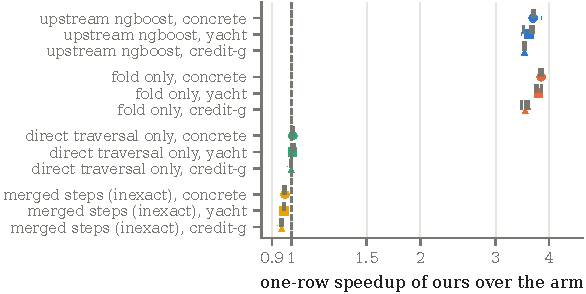
\includegraphics[width=0.95\linewidth]{figures/fig1_paired.pdf}
\caption{Ours beats upstream about 3.5 to 3.7 times for one row and ties direct traversal only, because tuned models hold no constant learner. Dots: speedup at $\bar d$; bars: two-level bootstrap 95\% interval; ticks: per-seed medians.}
\label{fig:paired}
\end{figure}

\textbf{Constant learners appear exactly where Lemma~\ref{lem:bound} says.} On the grid the constant share was never partial: \nGridDegenerateTotal{} of \nGridPointsTotal{} points were all-constant (concrete \nConcreteGridDegenerate, yacht \nYachtGridDegenerate, credit-g \nCreditGGridDegenerate), and these were precisely the points where the minibatch was below the split bound (Figure~\ref{fig:bound}). There one-row prediction was \nYachtGridDegMinX$\times$ to \nYachtGridDegMaxX$\times$ faster on yacht, \nConcreteGridDegMinX$\times$ to \nConcreteGridDegMaxX$\times$ on concrete and \nCreditGGridDegMinX$\times$ to \nCreditGGridDegMaxX$\times$ on credit-g; two yacht fits that upstream stopped after one round gained only \nYachtGridOneRoundMinX$\times$ to \nYachtGridOneRoundMaxX$\times$, since the gain scales with the rounds removed. The search never picks these points because they fit worse: held-out NLL \nConcreteGridDegNLL{} against \nConcreteGridBestNLL{} for the best concrete point, \nYachtGridDegNLL{} against \nYachtGridBestNLL{} on yacht.

\begin{figure}[H]
\centering
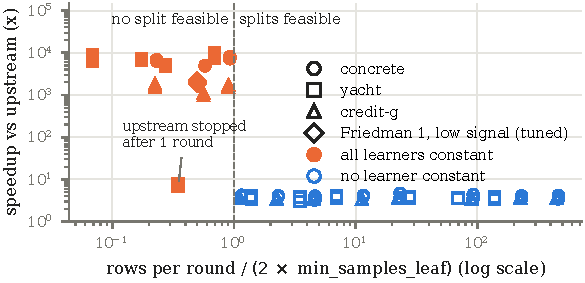
\includegraphics[width=0.95\linewidth]{figures/fig2_bound.pdf}
\caption{The split bound separates the two regimes: left of the line every learner is constant and folding gives three to four orders of magnitude; right of it no learner is constant and only direct traversal helps. One point per grid fit (one seed) and per low-signal fit.}
\label{fig:bound}
\end{figure}

\textbf{When does the search pick an all-constant model?} Only without usable signal. On Friedman's first benchmark function \citep{friedman1991mars} with the signal scaled down to pure noise and to a tenth of the noise (\nLowTrainRows{} training rows, \nLowTrials{} trials), the search picked leaf \nLowPickLeaf{} with minibatch \nLowPickMinibatch: \nLowBatchRows{} rows per round where \nLowMinRows{} are needed to split. Every learner was constant in all \nLowFits{} fits. One-row prediction dropped from \nLowPristineMinMs--\nLowPristineMaxMs{} ms upstream to \nLowOursMs{} ms, \nLowMinX$\times$ to \nLowMaxX$\times$ per fit (block-bootstrap SE of $d$ \nLowSEMin--\nLowSEMax, \nLowReps{} repetitions), bit-identical. Fold only was faster still, \nLowFoldMs{} ms, because the float32 cast of direct traversal is pure overhead there. The other two follow-ups did not reach the degenerate regime on their own. Credit-g cut to \nSmallTrainRows{} training rows picked depth \nSmallPickDepth, leaf \nSmallPickLeaf{} and \nSmallPickRounds{} rounds, constant share \nSmallShareMax\%, a \nSmallX$\times$ gain from direct traversal. The one-SE rule \citep{breiman1984cart} (pick the most regularised trial within one SE of the best) did choose all-constant models, but its held-out NLL was a tie with the best pick: \nOneSECGDiff{} $\pm$ \nOneSECGSE{} nats on credit-g ($n = \nOneSECGN$ test rows), \nOneSEFADiff{} $\pm$ \nOneSEFASE{} and \nOneSEFBDiff{} $\pm$ \nOneSEFBSE{} on the two Friedman levels ($n = \nOneSEFAN$).

\textbf{Outside the benchmark.} \nExternalLine

\section{Limits}
\label{sec:limits}

Folding gave no speedup on any tuned public model; the headline gain on those models is direct traversal, which is plain engineering on scikit-learn's call path. The large folding gains need a model with no usable signal, and such a model is better reported to the user than served faster: Lemma~\ref{lem:bound}'s warning may be the more useful part. The run is smaller than planned: \nDataSets{} data sets instead of the planned UCI suite, \nConcreteSeeds{} seeds, \nCVFolds-fold search, and no external speed reference such as compiled tree libraries \citep{cho2018treelite,nakandala2020hummingbird}. Building the plan costs \nConcretePlanOverFit\%, \nYachtPlanOverFit\% and \nCreditGPlanOverFit\% of fit time on concrete, yacht and credit-g (median), far above negligible on these small sets. Timings come from a shared host with load average \nLoadMin{} to \nLoadMax; the paired, interleaved design guards the ratios, not the absolute milliseconds. The benchmark SE uses only \nConcreteSeeds{} seeds and is two to three times smaller than the two-level SE; we report both. Folding zero-coefficient linear learners is exact only for finite inputs, so it is opt-in and was not benchmarked.

\bibliographystyle{plainnat}
\bibliography{refs}

\appendix

\section{Proofs}
\label{app:proofs}

\begin{proof}[Proof of Lemma~\ref{lem:fold}]
\textbf{Given:}
1) the upstream update, Equation~\eqref{eq:loop};
2) learner $(i,k)$ is constant: $f_{ik}(x) = v_{ik}$ for every row $x$ the model accepts;
3) IEEE~754 arithmetic: the result of $\fsub$ and $\fmul$ depends only on the two operands \citep{goldberg1991floating};
4) $1 \fmul a = a$ for every finite float $a$.

\textbf{Choose:} a column $k$, a row $x$ that upstream accepts, and the chain $c_0 = \theta_{0,k}$, $c_i = c_{i-1} \fsub s_{ik}$ for $i < i^*_k$, so $c_{i^*_k - 1} = \text{start}_k$ (Equation~\eqref{eq:start}).

\textbf{Need to prove:} $\theta_k^{(i)}(x) = c_i$ for all $i < i^*_k$. Assume it for $i-1$ (it holds for $i = 0$ by definition). Then
\begin{align*}
\theta_k^{(i)}(x) &= \theta_k^{(i-1)}(x) \fsub \big((\eta \fmul f_{ik}(x_{c_i})) \fmul \rho_i\big) && \text{given 1}\\
&= \theta_k^{(i-1)}(x) \fsub \big((\eta \fmul v_{ik}) \fmul \rho_i\big) && \text{given 2, round } i < i^*_k \text{ is constant}\\
&= c_{i-1} \fsub \big((\eta \fmul v_{ik}) \fmul \rho_i\big) && \text{induction assumption, given 3}\\
&= c_{i-1} \fsub s_{ik} = c_i && \text{definition of } s_{ik} \text{ and } c_i
\end{align*}
Folded prediction starts at $1 \fmul \text{start}_k = \text{start}_k$ (given 4), which equals $\theta_k^{(i^*_k - 1)}(x)$.

\textbf{Same method, but on rounds $i \ge i^*_k$.} Assume folded and upstream agree after round $i-1$. If $(i,k)$ is a tree step, folded applies Equation~\eqref{eq:loop} itself, with direct traversal in place of \texttt{predict}. If it is a scalar step,
\begin{align*}
\theta_k^{(i-1)} \fsub s_{ik} &= \theta_k^{(i-1)} \fsub \big((\eta \fmul v_{ik}) \fmul \rho_i\big) && \text{definition of } s_{ik}\\
&= \theta_k^{(i-1)} \fsub \big((\eta \fmul f_{ik}(x_{c_i})) \fmul \rho_i\big) && \text{given 2}
\end{align*}
which is the upstream update. Steps are kept in round order and never merged, so each side applies the same operation to the same operands (given 3).

\textbf{Precondition: direct traversal returns the same tree output.} Upstream \texttt{predict} casts $x_{c_i}$ to float32 and walks the tree; direct traversal casts the same columns to float32 once and walks the same nodes with the same thresholds. Same comparisons give the same leaf, and the same leaf gives the same stored float64 value.

\textbf{Precondition: given 2 holds on every accepted row.} A one-node tree stops at the root for any $x$; a tree whose leaves all hold $v_{ik}$ returns $v_{ik}$ whichever leaf $x$ reaches; a \texttt{DummyRegressor} ignores $x$. Rows that would make a skipped learner raise (NaN or infinity where it rejects them) are found by the probe on a zero, a NaN and an infinity row, and folded prediction rejects them too.

\textbf{Therefore,} by induction over $i = 1,\dots,M$, folded $\theta_k(x)$ equals upstream $\theta_k^{(M)}(x)$ bit for bit, for every $k$ and every accepted $x$.
\end{proof}

\begin{proof}[Proof of Lemma~\ref{lem:bound}]
\textbf{Given:}
1) a CART node \citep{breiman1984cart} as fitted by scikit-learn splits only if it holds at least min\_samples\_split rows and each child gets at least $L$ rows;
2) each round fits its trees on $m = \lfloor \phi\, n' \rfloor$ rows;
3) Lemma~\ref{lem:fold}.

\textbf{Choose:} any round $i$ and parameter $k$, and suppose the root of $f_{ik}$ splits into children with $m_\ell$ and $m_r$ rows.

\textbf{Need to prove:} a split requires $m \ge \max(\text{min\_samples\_split}, 2L)$.
\begin{align*}
m &= m_\ell + m_r && \text{every row goes to one child}\\
  &\ge L + L = 2L && \text{given 1, leaf condition}\\
m &\ge \text{min\_samples\_split} && \text{given 1, split condition}
\end{align*}
So if $m < \max(\text{min\_samples\_split}, 2L)$ the root cannot split and $f_{ik}$ is a one-node tree. $m$ is the same in every round, so this holds for all $i$ and $k$, and $i^*_k = M + 1$ for every column.

\textbf{Therefore,} by Lemma~\ref{lem:fold} with no tree step, $\theta_k(x) = \text{start}_k$ for every $x$: one fixed distribution. Under $K$-fold cross-validation $n'$ is the training-fold size, so the bound bites earlier during tuning than on the full data. The converse is not claimed: a feasible split can still be skipped when no split lowers the loss.
\end{proof}

\section{Environment and reproduction}
\label{app:env}

Python \nVerPython, ngboost \nVerNgboost, scikit-learn \nVerSklearn, numpy \nVerNumpy; one OpenMP thread per process; shared \nCores-core host, load average \nLoadMin--\nLoadMax; tuned runs took \nWallTuned{} s wall time. Grid: learning rate \nGridLR, \nGridRounds{} rounds, \nGridRepsOne{} one-row repetitions per point. Tuned picks: concrete depth \nConcretePickMaxDepth, leaf \nConcretePickMinSamplesLeaf, minibatch \nConcretePickMinibatchFrac, rate \nConcretePickLearningRate, \nConcretePickNEstimators{} rounds; yacht \nYachtPickMaxDepth, \nYachtPickMinSamplesLeaf, \nYachtPickMinibatchFrac, \nYachtPickLearningRate, \nYachtPickNEstimators; credit-g \nCreditGPickMaxDepth, \nCreditGPickMinSamplesLeaf, \nCreditGPickMinibatchFrac, \nCreditGPickLearningRate, \nCreditGPickNEstimators. Held-out NLL of the tuned models: concrete \nConcreteTunedNLL, yacht \nYachtTunedNLL, credit-g \nCreditGTunedNLL{} nats. Code: repository \texttt{ngbfast}, commit \texttt{\nCommit}; upstream patch \texttt{patches/ngboost-fold-constant-trees.patch}. Results: \texttt{python -m bench.summarize} after the per-data-set runs listed in \texttt{bench/results/SCOPE.md}; every number in this paper is a macro written by \texttt{paper/results/make\_numbers.py} from \texttt{bench/results/}.

Figure~\ref{fig:latency} gives the absolute one-row latency per arm.

\begin{figure}[H]
\centering
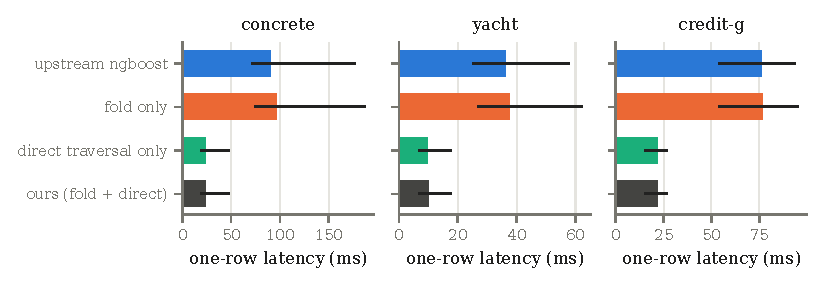
\includegraphics[width=0.95\linewidth]{figures/fig3_latency.pdf}
\caption{Direct traversal removes about three quarters of upstream's one-row latency; fold only is no faster than upstream on tuned models. Bars: median over all repetitions and seeds; lines: 10th to 90th percentile.}
\label{fig:latency}
\end{figure}

\end{document}
